\documentclass[aspectratio=169]{beamer}
\usepackage{spc}
\begin{document}

\begin{frame}
  \title{\darkblue Introduction to Git and GitHub}
  \author{\darkgray\bf Arni Magnusson\\
    \phantom{.}\h{32ex}
\includegraphics[width=1cm]{github_logo}}
  \date{\darkgreen SPC Git/GitHub Workshop\\[0.5ex]
    Noumea, 13 April 2022}
  \titlepage
\end{frame}

% ______________________________________________________________________________

\begin{frame}{Overview}
  \begin{itemize}
    \item[] {\bf\darkblue Examples}
    \comment{SPC software, analyses, information\\[1ex]
      \h{14ex}Fisheries software, open data, personal notes}\\[5ex]
    \item[] {\bf\darkblue Benefits}
    \comment{track changes, backups, collaboration, dissemination}\\[5ex]
    \item[] {\bf\darkblue Git concepts}
    \comment{repositories, commits, tags, branches, gitignore}\\[5ex]
    \item[] {\bf\darkblue GitHub features}
    \comment{releases, assets, forks, pull requests, issues,\\[1ex]
      \h{21.4ex}access control, authentication}\\[1ex]
  \end{itemize}
\end{frame}

% ______________________________________________________________________________

\begin{frame}\Large
  \centering\darkgreen\bf
  GitHub Examples
\end{frame}

% ______________________________________________________________________________

\begin{frame}[plain]
  \begin{tikzpicture}[remember picture,overlay]
    \node[at=(current page.center)]
    {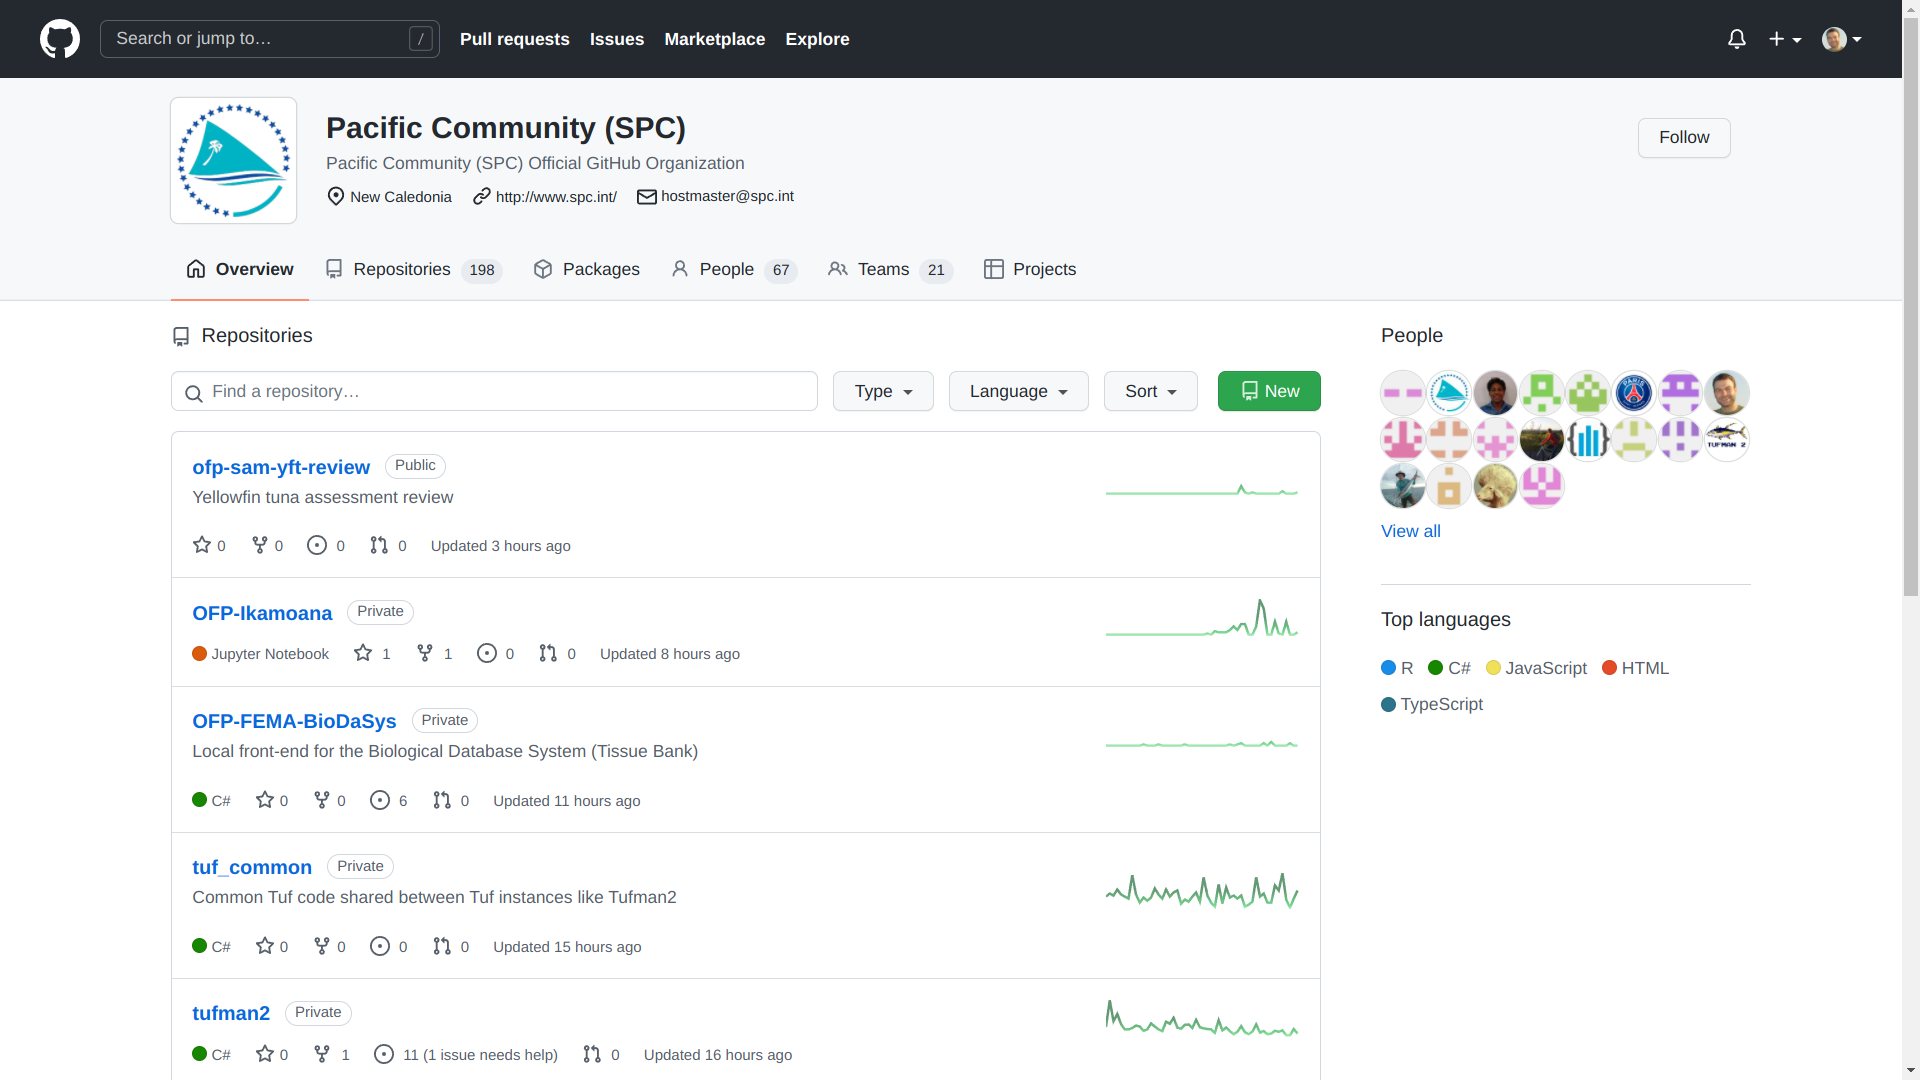
\includegraphics[width=\paperwidth]{github_spc}};
  \end{tikzpicture}
\end{frame}

% ______________________________________________________________________________

\begin{frame}{GitHub Repositories}\small
  \begin{description}
    \item[\bf\green SPC software]
    \href{https://github.com/PacificCommunity/tufman2}
    {\darkblue TUFMAN2},
    \href{https://github.com/PacificCommunity/ofp-md2}
    {\darkblue MD2},
    \href{https://github.com/PacificCommunity/ofp-sam-mfcl}
    {\darkblue MFCL},
    \href{https://github.com/PacificCommunity/ofp-sam-mfcl-viewer}
    {\darkblue MFCL viewer},
    \href{https://github.com/PacificCommunity/ofp-sam-flr4mfcl}
    {\darkblue FLR4MFCL},
    \href{https://github.com/PacificCommunity/ofp-sam-latex-utils}
    {\darkblue LaTeX utilities}\\[4ex]
    \item[\bf\green SPC analyses]
    \href{https://github.com/PacificCommunity/ofp-sam-cpue2021}
    {\darkblue CPUE analysis},
    \href{https://github.com/PacificCommunity/ofp-sam-yft-2020-runs}
    {\darkblue Yellowfin 2020 assessment},
    \href{https://github.com/PacificCommunity/ofp-sam-skj22}
    {\darkblue Skipjack 2022 assessment}\\[4ex]
    \item[\bf\green SPC information]
    \href{https://github.com/PacificCommunity/ofp-sam-yft-review}
    {\darkblue Yellowfin review},
    \href{https://github.com/PacificCommunity/ofp-sam-htcondor}
    {\darkblue Condor tutorial},
    \href{https://github.com/PacificCommunity/ofp-sam-institutional-memory}
    {\darkblue Condor notes},
    \href{https://github.com/PacificCommunity/ofp-sam-taf-demo}
    {\darkblue TAF demo}\\[4ex]
    \item[\bf\green Fisheries software]
    \href{https://github.com/admb-project/admb}{\darkblue ADMB},
    \href{https://github.com/kaskr/adcomp}{\darkblue TMB},
    \href{https://github.com/James-Thorson-NOAA/VAST}{\darkblue VAST},
    \href{https://github.com/fishfollower/SAM}{\darkblue SAM},
    \href{https://github.com/gadget-framework/gadget2}{\darkblue Gadget},
    \href{https://github.com/NIWAFisheriesModelling/CASAL2}{\darkblue CASAL},
    \href{https://github.com/nmfs-stock-synthesis/stock-synthesis}
    {\darkblue Stock Synthesis},
    \href{https://github.com/ices-tools-prod/TAF}{\darkblue TAF}\\[4ex]
    \item[\bf\green Open data~~~]\h{-3ex}
    \href{https://github.com/cfree14/wcfish}{\darkblue US West Coast fisheries},
    \href{https://github.com/CSSEGISandData/COVID-19}
    {\darkblue Covid data}\\[4ex]
    \item[\bf\green Personal notes]
    \href{https://github.com/arni-magnusson/corona}{\darkblue Covid analysis},
    \href{https://github.com/arni-magnusson/dot}
    {\darkblue Computer settings}\\[1ex]
  \end{description}
\end{frame}


% ______________________________________________________________________________

\begin{frame}\Large
  \centering\darkgreen\bf
  Benefits of Using Git and GitHub
\end{frame}

% ______________________________________________________________________________

\begin{frame}{Benefits of Using Git/GitHub}\small
  \begin{description}
    \item[\bf Track changes] Who changed what, when, and why\\[5ex]
    \item[\bf Backups] Online\\[1ex]
    Restore previous state\\[5ex]
    \item[\bf Collaboration] Local, regional, international\\[1ex]
    \h{1ex}Software development, analyses, other projects\\[5ex]
    \item[\bf Dissemination] Software\\[1ex]
    \h{1.5ex}Open science, data hub\\[1ex]
    \h{1.5ex}Products\\[1ex]
  \end{description}
\end{frame}

% ______________________________________________________________________________

\begin{frame}\Large
  \centering\darkgreen\bf
  Git Concepts
\end{frame}

% ______________________________________________________________________________

\begin{frame}{Git Concepts}\small
  \begin{description}
    \item[\bf Repository] Online folder, Who changed what, when, and why\\[5ex]
    \item[\bf Commit] Saved state\\[5ex]
    \item[\bf Tag] Local, regional, international\\[5ex]
    \item[\bf Branch] Software, open science\\[5ex]
    \item[\bf Gitignore]
  \end{description}
\end{frame}

\end{document}
